\documentclass[a4paper, oneside]{memoir}
\usepackage[top=25mm, bottom=25mm]{geometry}	% layout margin
\usepackage{graphicx}
\graphicspath{ {./images/} }

\title{Report for the Project of Distributed Systems}

\author{Ermacora Gianluca 132923\\ Rovere Andrea 128074}

\date{\today}

\begin{document}


\begin{titlingpage}
\maketitle
\begin{abstract}
The goal of this project is the creation of a network of drones to satisfy the delivery requests of clients, the drones, the client and all the other entities required for the proper operation of the system will be implemented in Erlang.
\end{abstract}
\end{titlingpage}

\chapter{Introduction}\label{ch:intro}

%In this chapter you describe the main problem, and an idea of the solution. It is not necessary to be very detailed or formal, but it is important to explain which are the main aims and issues from the point of view of Distributed Systems:
%\begin{itemize}
%A description of the application.
%The overall structure of the implementation: how resources are deployed, which are the players, the roles.
%\item The distributed system features (and the transparencies) and algorithms you intend to implement.
%\item Your plan for testing the system.
%\item A schedule for how you plan to carry our your design and implementation
%\end{itemize}

\section{Description of the application.}
The problem to solve is the delivery of packages and management of a dynamic fleet of drones.

The space is modelled by a 2D grid, so the diagonal movements of drones are calculated with some approximation. There aren't forbidden zones nor forced paths.

The drones have cellular connectivity and know a few other drones. They are equipped with GPS and we assume they have an ID, it's not a limitation since the ID could be given by the manager server (see below).

There are some recharging and repairing stations on the map. For simplicity the recharging stations and warehouses are assumed to have unlimited capacity.

There is a server that centralize the orders of the clients and act as a reliable message broker (as middle-man).

There is a server which provide some management of drones, and make sure the order is carried out. In particular, the tracker functionality, when a new drone is connected the server will provide a list of other drones to connect to and the locations of recharging/repairing stations.

The two servers are separated due to the fact that we are following the principle of separation of concerns, and because in case of multiple fleets of drones we would have one broker and various manager servers.

\begin{figure}[h!]
	\centering
	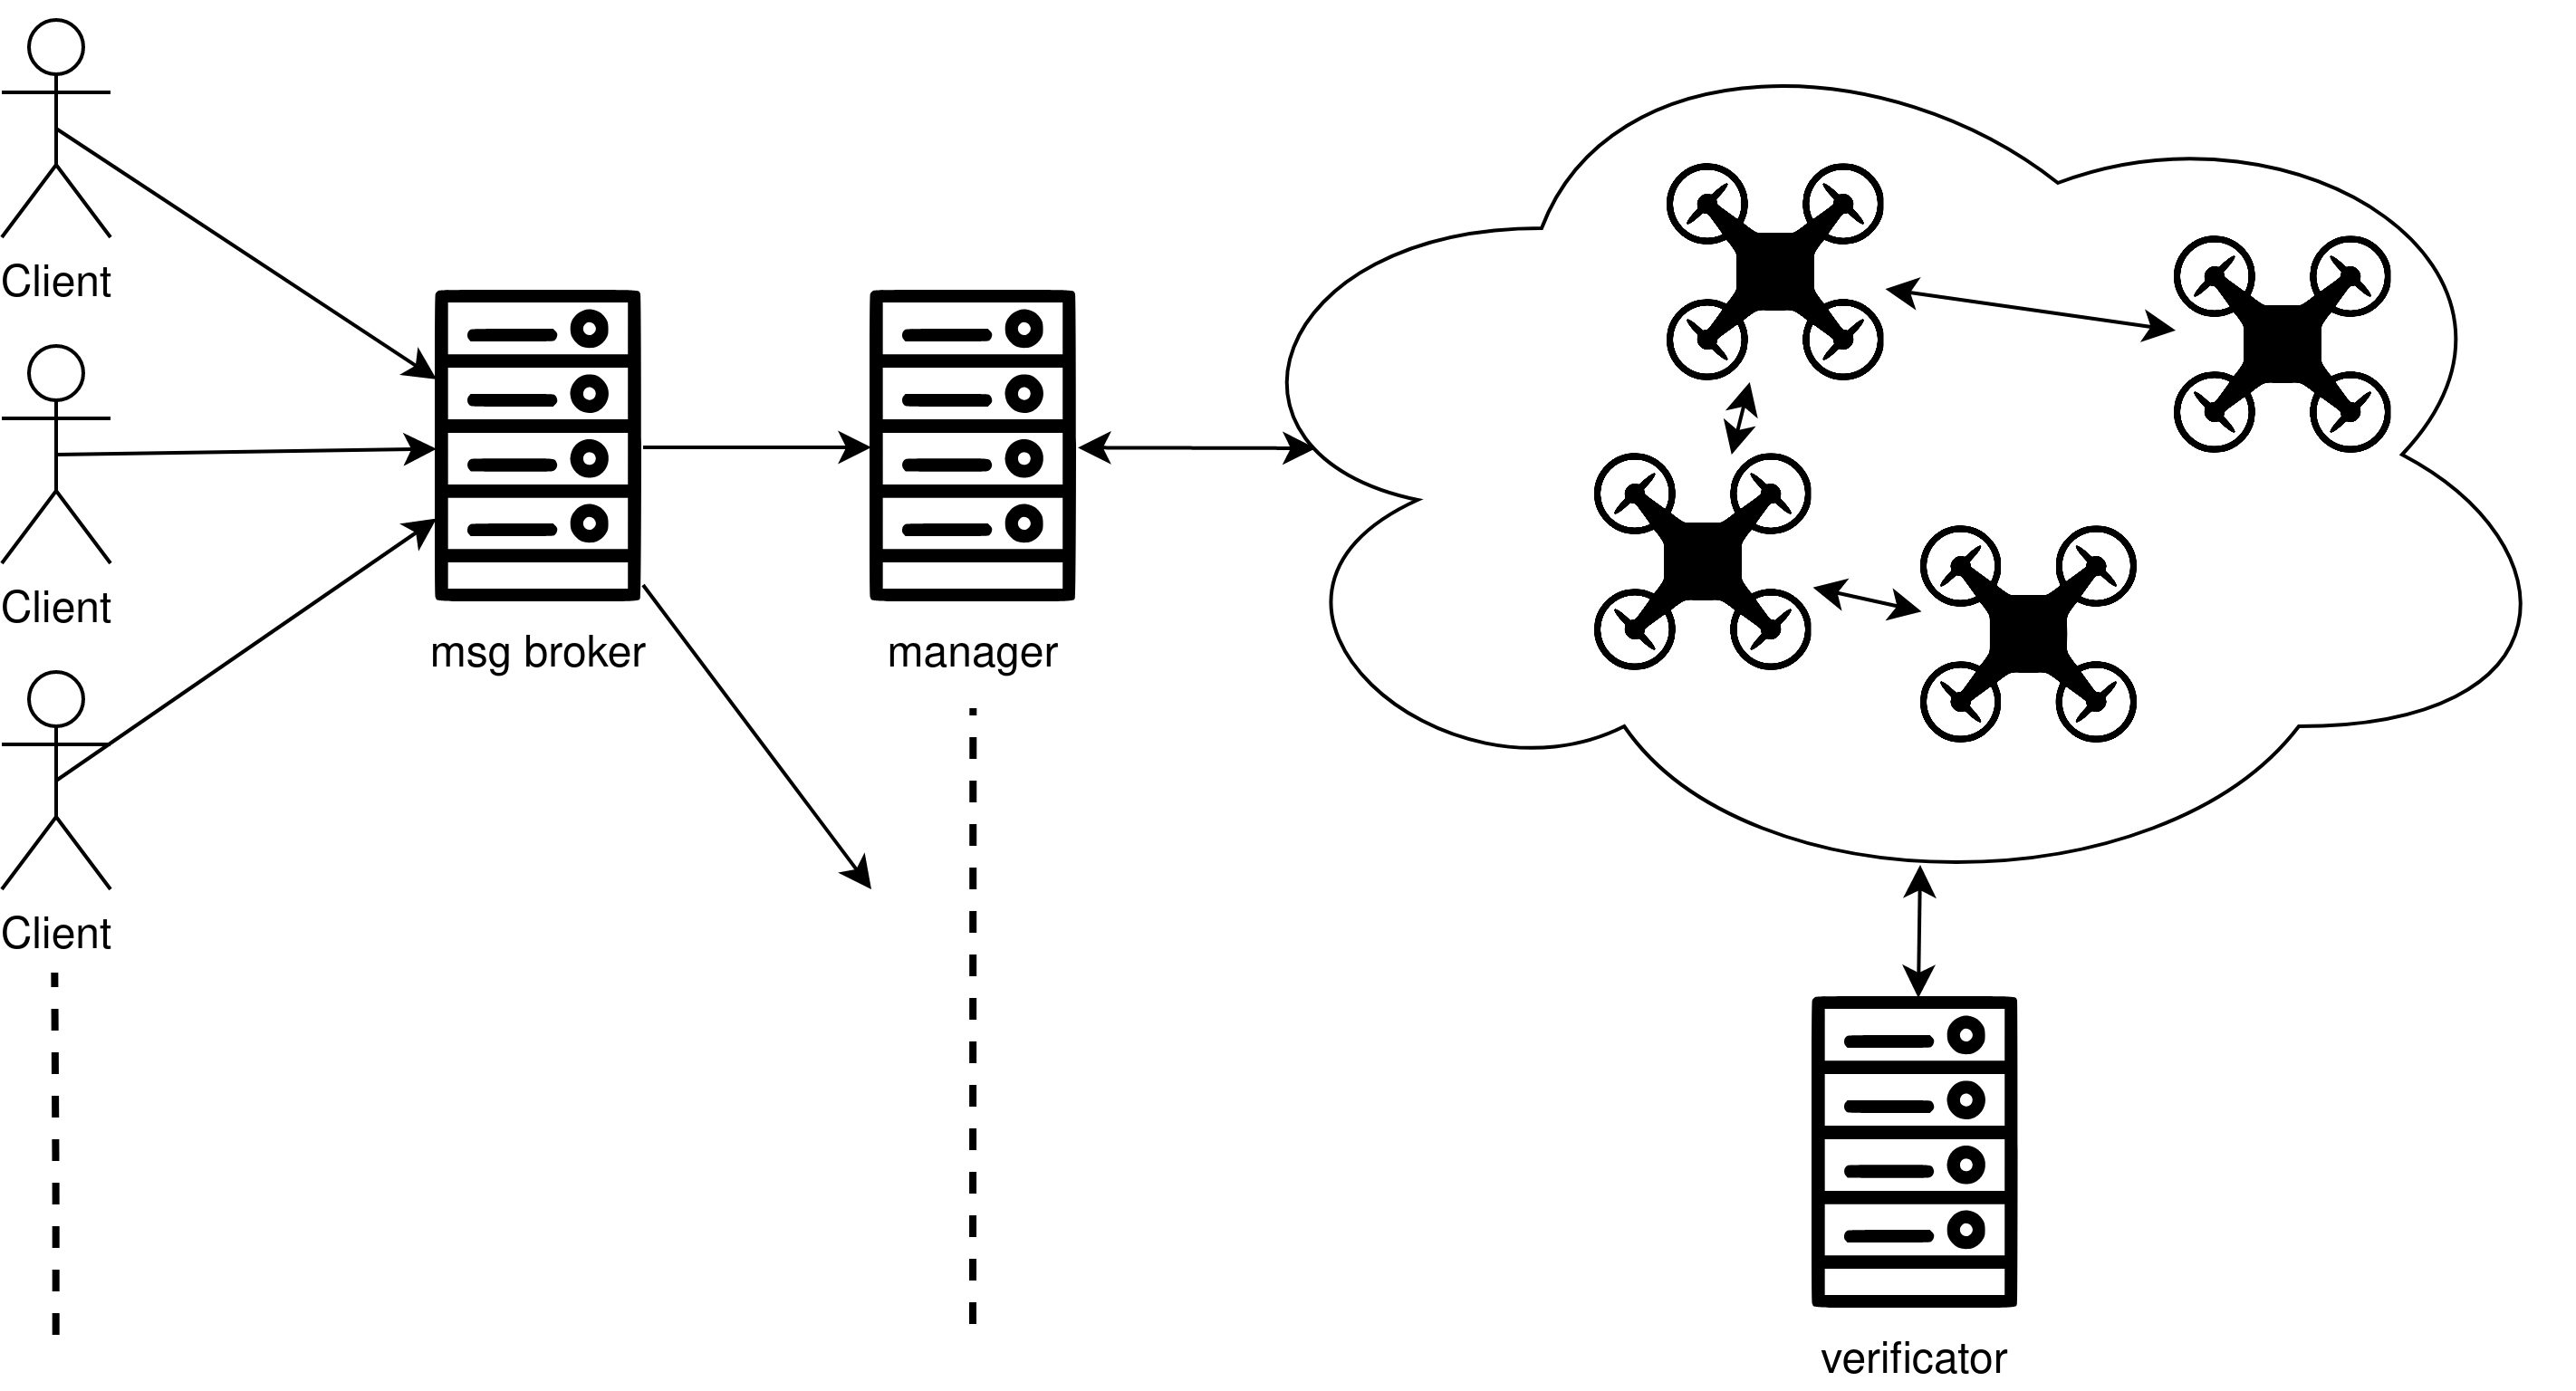
\includegraphics[width=\linewidth]{Overview}
\end{figure}

A client can send a request to the broker server for the delivery of a package from point A to point B, a drone will be selected based on its position relative to point A, its  battery and maximum carry weight, the selected drone will carry out the delivery of the package.

If a drone has low battery it will enter reserve mode, it will locate the nearest charging station and it will move in that direction, the charging stations are fixed and their location is known to all drones. After a drone refused three orders due to the low battery, it will go to the recharging station, this will mitigate but not prevent the refuse of a package by the fleet; the manager will handle the case.

A drone can crash at any point in time, if it was able to signal the fail, another drone will be selected to transport the broken drone to the nearest charging station, if the broken drone was satisfying a request a second drone will be selected to complete the task.


\section{Structure of the implementation}

The client position is not considered in our system, drones can be in any point in the map and move only if they need to deliver a package or if they need to recharge, the charging stations are located in fixed points in the map, their position is known to all drones.

The key players in our implementation are:
\begin{itemize}
\item \textbf{Client}: the client sends a request to the broker server for a delivery. It's also able to query the broker asking for the status of the delivery;
\item \textbf{Drone}: the drones are the entities that move the packages between locations, new drones that want to join the network send a message to the manager server, drones with low battery must go to a charging station to recharge;
\item \textbf{Broker server}: this server receives the requests from clients, it's a single point of failure so it is replicated by a backup copy (it's possible to have more copies);
\item \textbf{Manager server}: this server handles the join of a new drone in the network, a drone can have it's own unique id or can obtain one from this server. Other functionalities are the detection of an offline drone and consequentially offers the best-effort guarantee of successful delivery. The server is a single point of failure so it is replicated by a backup copy (it's possible to have more copies);
\item \textbf{Recharging/Repairing station}: these are stations in fixed points in the map where drones can go to recharge their battery and where broken drones can be brought for repairs.
\end{itemize}


\section{System features}

The system transparencies that we aim to implement are:
\begin{itemize}
	\item \textbf{concurrency transparency}: only one drone will be selected to carry out the delivery of a package, but multiple orders from multiple clients are handled concurrently;
	\item \textbf{failure transparency}: if a drone crashes the delivery must be completed smoothly for the client, if the broker server or the manager server crash the systems will connect to a secondary backup server;
	\item \textbf{location transparency}: the position of the drones is unknown to the clients;
	\item \textbf{performance and scaling transparency}: the system must be able to scale smoothly when adding more drones;
	\item \textbf{reconfiguration transparency}: the entrance of a new drone in the network must have a low overhead.
\end{itemize}

\subsection{Assumption}
We utilized the simplify assumption that the channels offer reliable delivery without data duplication. This isn't an unrealistic assumption since we can imagine to transfer data packets (UDP) over an overlay TCP network.

\subsection{Election Algorithm}
For the election of the drone we firstly considered the "Bracha-Toueg fail consensus algorithm", then the "Echo with extinction", then we reached the conclusion that also the "Echo" would work. The "Bracha-Toueg" was discarded because it needs to know the size of the network (N), this means that the manager needs to calculate and distribute the size. The other problem was that the "Bracha-Toueg" needs a major modification which consists in making sure that the majority of the network converges to the minimum distance known by the network.

The differences between the "Echo" and "Echo with extinction" are that: in the "Echo" the algorithm has a single initiator, that makes the last decision in the election, which needs to be broadcasted; while in the "Echo with extinction" the initial node is really a propagator of the request for all the nodes start a wave, so this initial node make the broadcast of the order and when the execution terminates the elected node knows that is elected.

The message complexity for the "Echo" algorithm is $2M$ plus the propagation complexity of the decision $O(M)$ where $M$ is the number of edges in the network. So the total complexity is $ O(M) $.
Instead the message complexity for the "Echo with extinction" is $O(M)$ for the initial broadcast and then $O(N M)$ for the algorithm.

The decision is obvious: the "Echo" is the better choice in the worst case. The drawback is that the failure of a drone during an election will block the election; this situation is mitigated by the manager that will restart the election while if a drone doesn't respond it will be removed from the list of neighbours on the drones involved. The "Echo" has been chosen because the manager have to handle the generic failure of a drone, and the failed election is a just particular case.

The "Echo" algorithm has been chosen due to the lower message complexity, that's because a comparison of the performance of the two algorithm over multiple election, in real cases, over a realistic network topology, is outside the scope of this project.

Simplification: under the assumption that the drones can reach each other, the communication of the decision of the election algorithm is made by a single message from the initiator node to the elected node.

Note: the criterion used for the decision of the node is based on distances instead of IDs, the IDs are used only in case of conflict due to same distance.


\section{Test cases}

To test our system we'll use a program that simulates the environment and spawns clients in random positions and with random requests, each entity in our system will run on a different virtual machine to better simulate the distributed aspects of our system.

The test cases that have been analysed are listed below:\\

Normal conditions:
\begin{itemize}
	\item the case where a drone successfully completes a delivery request;
	\item the case where a drone has to go to a charging station;
	\item the case where a new drone joins the network;
\end{itemize}

Critical situations:
\begin{itemize}
	\item the case where a drone crashes while it's idle;
	\item the case where a drone crashes after it has been selected to move a package but it has not picked up the package yet;
	\item the case where a drone crashes after it has picked up the package and it's delivering it to point B;
	\item the case where a drone has low battery power;
	\item the case where a drone is out of battery power due to misreading of the sensor or strong wind;
	\item the case where a drone crashes after it has sent its features(battery, position and carry weight) to the network for election;
	\item the case where no drone is available to deliver a package;
	\item the case where a drone crashes during the join request to the manager server.
\end{itemize}


\section{Schedule for the design and implementation of the system}
The schedule for how you plan to carry our your design and implementation is as follows:
\begin{enumerate}
\item Design of the system and definition of the functional and non-functional requirements;
\item Selection of the programming language for the implementation;
\item Specification of the protocols and algorithms that are used in the system;
\item Implementation of the entities that play a role in the system and the communication between them;
\item Testing of each part of the system and the system as a whole;
\end{enumerate}

\chapter{Analysis}\label{ch:analysis}

%In this chapter, we describe in detail functional and non-functional requirements of a solution for the problem.

\section{Functional requirements}

%Which functions must be offered to users / other programs?  Which are the input data and the output data? Which is the expected effect?

The following are the functional requirements required by the project:
\begin{itemize}
\item \textbf{Make a delivery request}: a client can request the delivery of a package form point A to point B.

	\textbf{Input}: the package starting position, the destination and the weight of the package;

	\textbf{Output}: there is no output;

	\textbf{Effect}: the election of a drone.

\item \textbf{Request for the status of a delivery}: the client can request the status of it's request to the broker server.

 	\textbf{Input}: the identification number for the order;

	\textbf{Output}: a message to the client signalling the status of the delivery;

	\textbf{Effect}: letting the client know about the status of the delivery.

\item \textbf{Support for a crashed drone while it is idle}: a drone that crashes while idle can request to be taken to a repair station,

	\textbf{Input}: the broken drone position;

	\textbf{Output}: there is no output;

	\textbf{Effect}: the election of a drone that will move the broken drone to a repair station.

\item \textbf{Support for a broken drone after it has been elected}: a drone that crashes after it has been chosen can request to be taken to a repair station.

	\textbf{Input}: the broken drone position and whether or not it picked up the package;

	\textbf{Output}: there is no output;

	\textbf{Effect}: the effect is the election of a drone that will move it to a repair station and the election of another drone to carry out the delivery.

\item \textbf{A new drone joins the network}: a new drone that wants to join the network sends a message to the management server.

	\textbf{Input}: the new drone unique id if he has one, its carry weight and its position;

	\textbf{Output}: the unique id(if needed) and the other drones to connect to;

	\textbf{Effect}: the entrance of the new drone in the network and the update of the manager drone table and the drones neighbout lists.

\item \textbf{Election of a drone to carry out a task}: a drone will be selected based on its characteristics and its position to carry out a task 

	\textbf{Input}: the drone table and the task to do;

	\textbf{Output}: the selected drone or an error message if one can't be selected;

	\textbf{Effect}: the selection of a specific drone to carry out a delivery or to move a broken drone to a repair station.

\end{itemize}

\section{Non functional requirements}

%Everything about mode and transparencies: availability, mobility, security, fault tolerance, etc.
%Are there execution time bounds? Minimum data rates?
%If requested, specific platforms/languages/middlewares requirements for the implementation can be decided here. (E.g.: if the project is on a SOA, we may request that functions are offered via SOAP or RESTful services).

The following are the non-functional requirements required by the project:
\begin{itemize}
\item there is no limit on the minimum weight of a package but it can't weigh more than 1500 grams ;
\item there are no restrictions on the movements of the drones through the map or their position on the map;
\item there are no restrictions on the position of the source or destination of the delivery request;
\item it is not required to consider security problems or Byzantine behaviour the drones;
\item the system must be able to recover from the failure of a drone or a server;
\item a drone has to respond to messages from other drones or the management servers within 10 seconds or it will be considered dead;
\item it's important for following transparencies to be present:
	\begin{itemize}
	\item \textbf{concurrency}: only one drone will be selected to carry out the delivery of the package;
	\item \textbf{reconfiguration}: the entrance of a new drone in the network must have a low overhead;
	\item \textbf{failure}: if a drone crashes the delivery must be completed smoothly for the client;
	\item \textbf{performance and scaling}: the system must be able to scale smoothly when adding more drones;
	\item \textbf{location}: the position of the drones is unknown to the clients.
	\end{itemize}
\end{itemize}


\chapter{Project}
In this chapter we'll describe the logical architecture of our system, the structure of the messages exchanged in our system, the algorithms used and we'll explain in detail the most important functions of our system.
%This chapter is devoted to the description of the general architectures, and specific algorithms.

\section{Logical architecture}
%Describe the components of your systems: modules/objects/components/services. For each component, describe the functionalities it implements, and by who is used.
\subsection{Modules used in the implementation}
The Erlang modules used in the implementation of the system are:
\begin{itemize}
\item \textbf{broker.erl}: this module contains all the functions needed by the broker server to handle the delivery requests and to communicate them to the management server and to handle the query requests from the clients;
\item \textbf{client.erl}: this module contains all the functions needed by the client to make a delivery request and to query the status of its delivery;
\item \textbf{drone.erl}: this module contains all the functions needed by the drone to exchange messages with other drones for the election and with the management server to start the election and to update the status of the delivery;
\item \textbf{election.erl}: this module contains all the functions needed to elect a drone for the delivery and to exchange messages with the drones to achieve this goal;
\item \textbf{enviroment.erl}: the role of this module is to set up the broker and the manager servers and to spawn the clients and the drones;
\item \textbf{manager.erl}: this module contains all the functions needed by the manager server to handle the join of a new drone, to start the election procedure and to update the relative drone table and order status;
\item \textbf{utils.erl}: this module contains some functions that are useful for multiple other modules.
\end{itemize}


\subsection{Primary backup schema}
Since the broker and the manager servers are both single point of failure, it has been chosen to implement a backup for them. The schema used is the simplest: one primary and one backup.

After some experiments it has been chosen to handle the messages received by the servers, (broker and manager) in the following way: the backup server keeps pinging the primary. When the acting primary receives a message related to the orders of the clients it start a new Erlang process to handle the message. This new Erlang process contacts the backup server which create an other Erlang process. The two new processes synchronize the status of the order between the primary and backup server.

This approach permits an efficient use of the resources since it prevents blocking, allows to handle a vast number of messages thanks to the lightweight Erlang processes. Moreover when a fail happened it will disrupt only a small step of the execution of an order,instead of the entire server.


\section{Protocols and algorithms}
%Communication between components.


\subsection{Status of the order}
The delivery order from the client can be in one of the following status:
\begin{itemize}
\item \textbf{inProgress}: an order is in this state after the order message has been reliably store by the manager;
\item \textbf{inDelivery}: an order is in this state after the information about the elected drone has been reliably store by the manager;
\item \textbf{delivered}: an order is in this state after the package has been delivered to it's destination and the manager server receives the "delivered" message form the drone.
\end{itemize}


\subsection{Messages: formats and effects}

From client to broker
\begin{itemize}
	\item New order: "\{makeOrder, ClientAddress, ClientID, OrderID, \{Source, Destination, Weight\}\}".
	Source and Destination are tuples {X, Y} referring to the starting location and the destination location of the package, Weight refers to the weight of the package. The broker acknowledge it with "confirmedOrder" when the order has been reliably saved.

	\item Query order: "\{queryOrder, ClientAddress, ClientID, OrderID\}". The broker replies with "orderNotPresent" if there is no order with the given OrderID and ClientID or with the status of the order.
\end{itemize} \vspace{1em}
From broker to manager
\begin{itemize}
	\item New order: "\{makeOrder, ClientAddress, ClientID, OrderID, \{Source, Destination, Weight\}\}".
	This is the message received from a client, by the broker; the manager will reliably store it and it will reply with "\{inProgress, \{\}, ClientID, OrderID, \{\}\}".
\end{itemize} \vspace{1em}
From manager to broker
\begin{itemize}
	\item Update of an order: "\{Type, \{\}, ClientID, OrderID, \{\} \}".
	Where the type of the message is the status of the order, which can be inProgress, inDelivery, delivered. The broker will reliably store the new status without replying to the manager.
\end{itemize}\vspace{1em}
From manager to drones
\begin{itemize}
	\item New order: "\{makeOrder, ClientAddress, ClientID, OrderID, \{Source, Destination, Weight\}\}".
	This is always the original message, the random drone will start the election without notify the manager.

	\item Drone status:

	\item Order status:

	\item List of drones: "List". The message contains the list of new neighbours drones.
\end{itemize} \vspace{1em}
From drones to manager
\begin{itemize}
	\item Election result: "\{inDelivery, DroneID, ClientID, OrderID, \{\} \}".

	\item Election failure due to weight: "\{excessiveWeight, \{\}, ClientID, OrderID, \{\} \}".
	The election failed, for the current order, because there wasn't an available drone with sufficient carry capacity.

	\item Package delivered: "\{delivered, DroneAddress, ClientID, OrderID, \{\} \}".
	The drone will send the message to the manager which will reliably store it. The manager will reply with "confirmDelivered", and will notify the broker.

	\item Registration:  "\{joinRequest, DroneAddress, DroneID, \{MaxCarry\}, \{\} \}".
	The drone will send the message to the manager to express it's interest in joining the network, the manager will respond with a list of drones for it to connect to.

	\item Failure:  "\{failureNotification, DroneAddress, DroneID, \{\}, \{\} \}".
	The drone will send the message to the manager informing it of the drone failure.
\end{itemize} \vspace{1em}
From drones to drones
\begin{itemize}
	\item Echo election propagation: "\{election, HandlerAddress, ClientID, OrderID, \{Source, Destination, Weight\}\}".
	This message is sent in the first phase of the election.

	\item Echo election back-propagation: "\{result, ElectedDroneID, ElectedPid, Distance, \{ClientID, OrderID\} \}".
	This message is sent in the second phase of the election to the designed parent.

	\item Echo election notification: "\{elected, ClientID, OrderID, Source, Destination \}".
	This message is sent from the initiator to the elected node to inform it of the result.
\end{itemize}
\newpage


%UML sequence diagrams go here.
\textbf{Join of a new drone}

The Join of a new drone in the network follows the following steps:
\begin{enumerate}
\item  The drone that wants to join the network sends a message to the management server indicating its drone id and its maximum carry weight;
\item the management server saves the characteristics of the drone and responds with a list of drones;
\item the drone sends a connect message to each drone in the list given by the management server;
\item every drone contacted responds with an ack message,
\item every time the new drone receives an ack message it will add that drone to its neighbour list.
\end{enumerate}

\begin{figure}[h!]
	\centering
	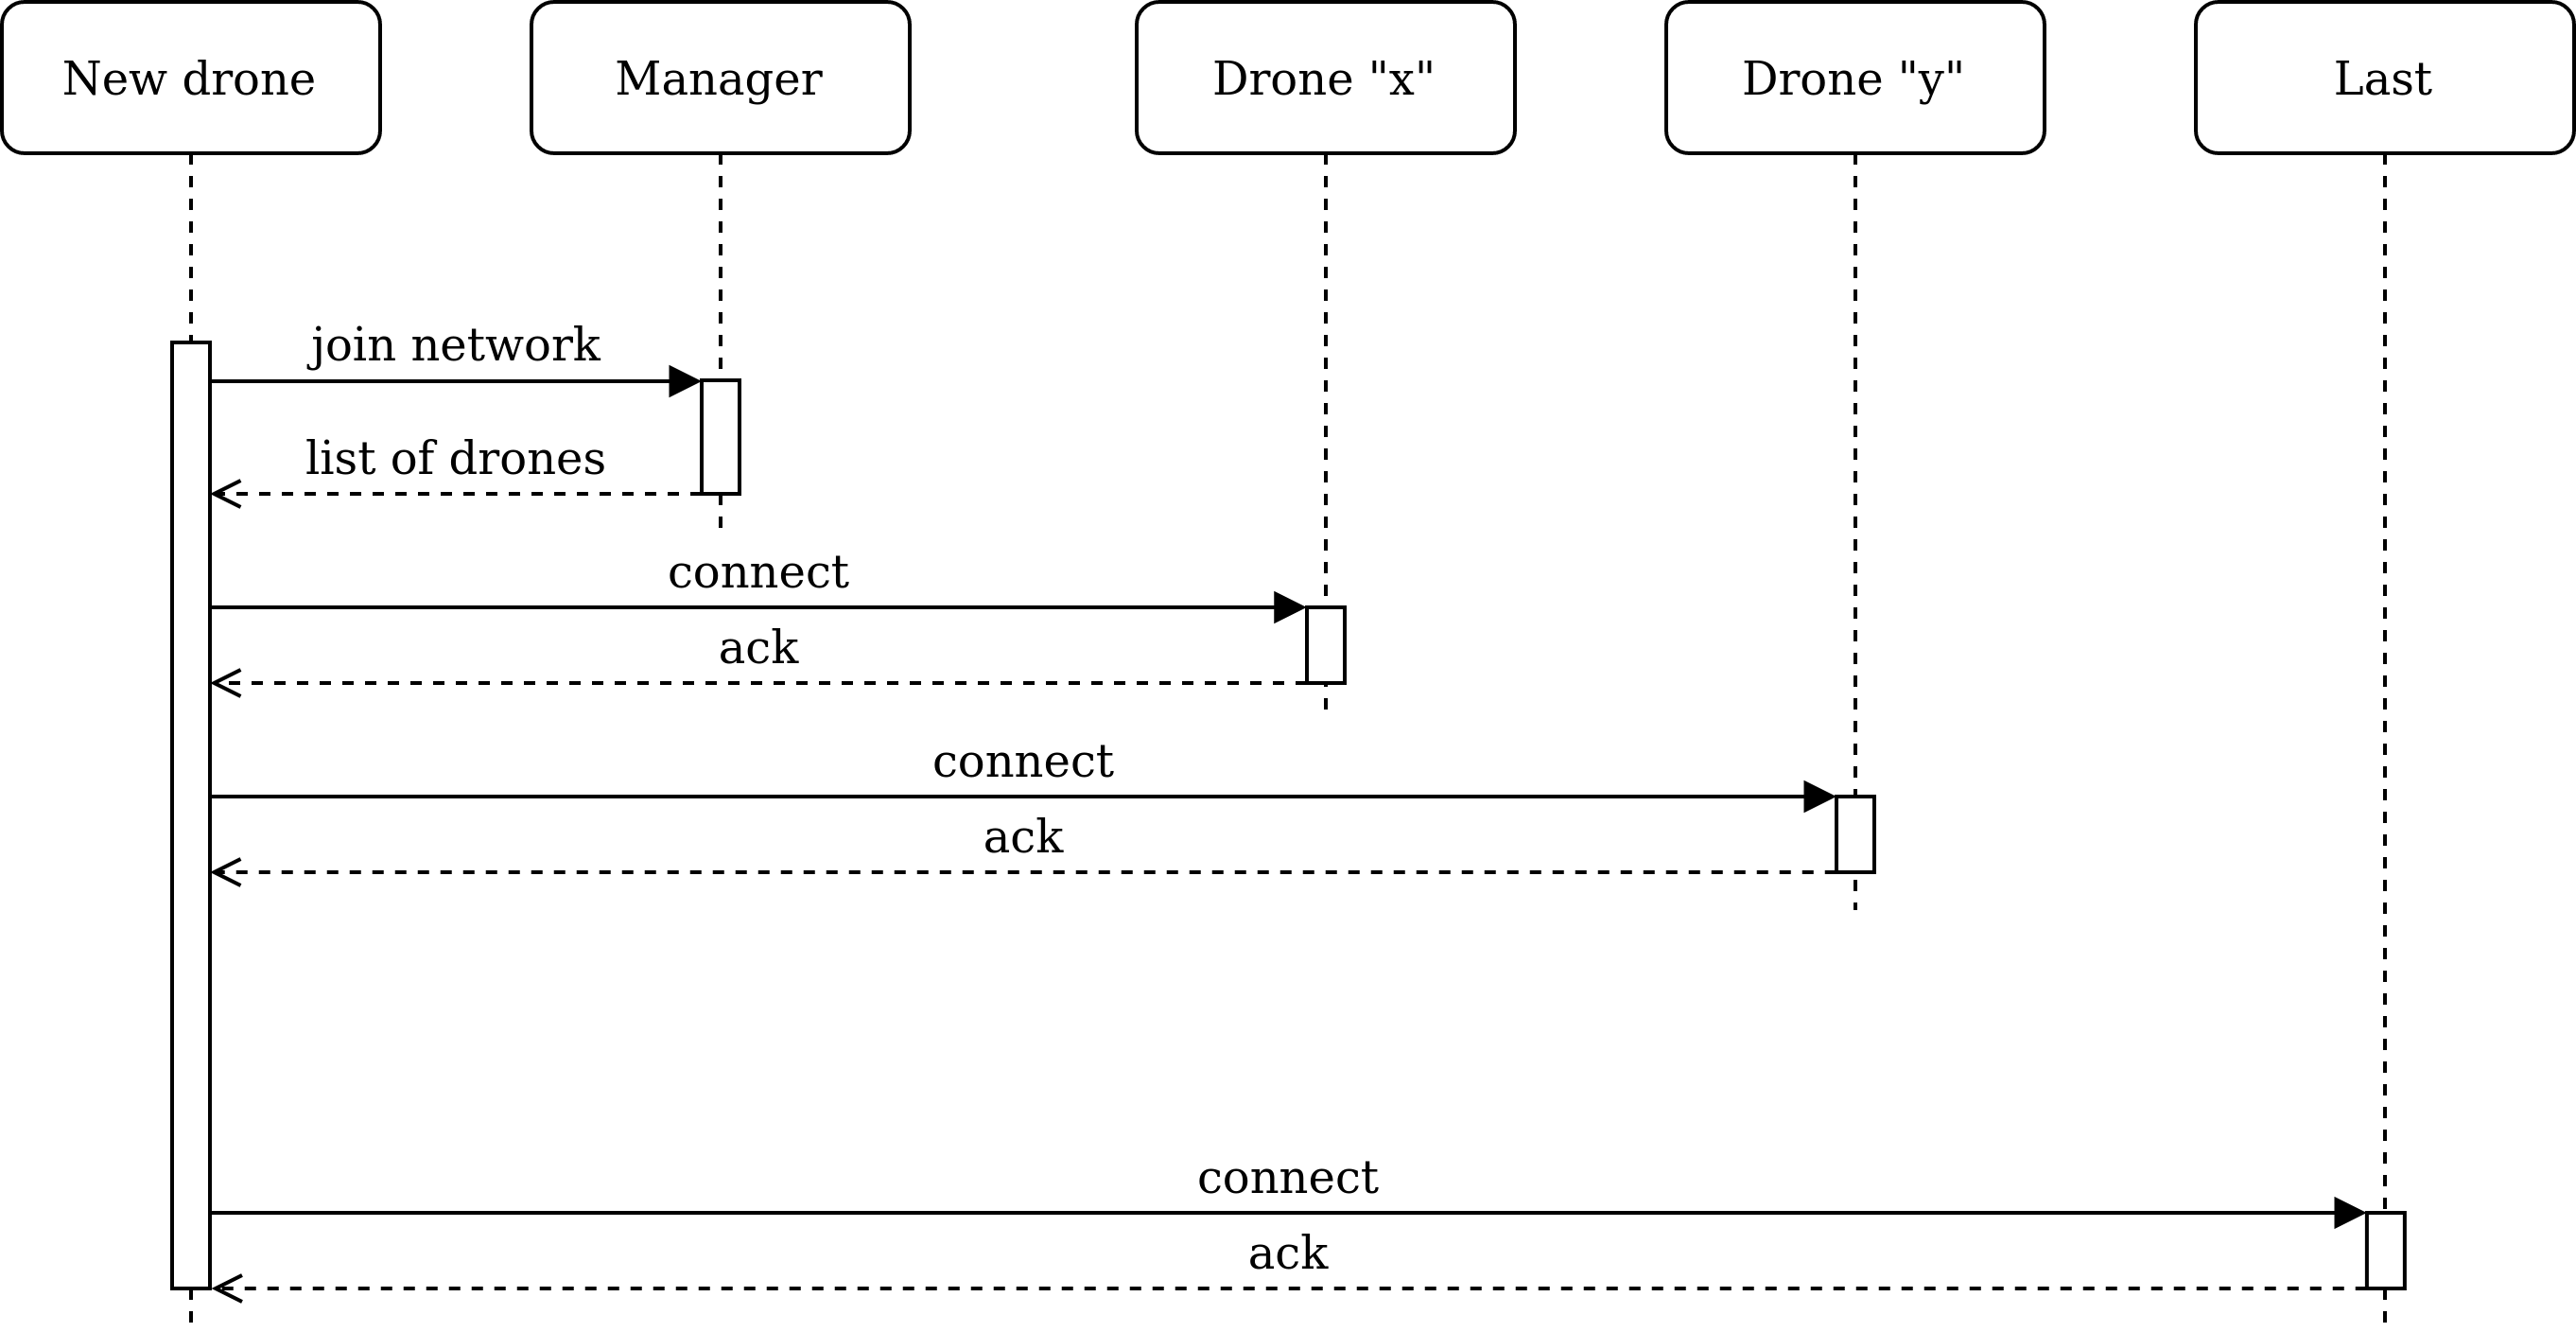
\includegraphics[width=\linewidth]{New-drone}
	\caption{UML diagram for the join of a new node }
\end{figure}


\textbf{New delivery request}

The execution of a new delivery request follows the following steps:
\begin{enumerate}
\item The client sends a message to the broker server with the delivery request;
\item the broker server saves the order, then it sends back an ack message to the client, finally it delivers the request to the manager server;
\item once the manager server receives the request, it stores the order then replies to the broker server with the message "inProgress" which is equivalent to an ack, then it selects a random drone and delivers the request to it;
\item the chosen drone initiates the election procedure and exchanges the necessary messages with other drones;
\item once a drone has been selected to carry out the delivery it sends a message to the manager server informing it of the result of the election;
\item the manager server notifies the broker server of the new status of the delivery;
\item the selected drone carries out the delivery and once it deposits the package at the destination it sends a message to the manager server updating the status of the delivery;
\item the manager server saves the new status of the delivery, responds with an ack to the drone and sends a message to the broker server updating the status of the delivery;
\item at any point the client can send a message to the broker server with a query for the status of its delivery;
\item the broker server responds with a message containing the status of the request.
\end{enumerate}

\begin{figure}[h!]
	\centering
	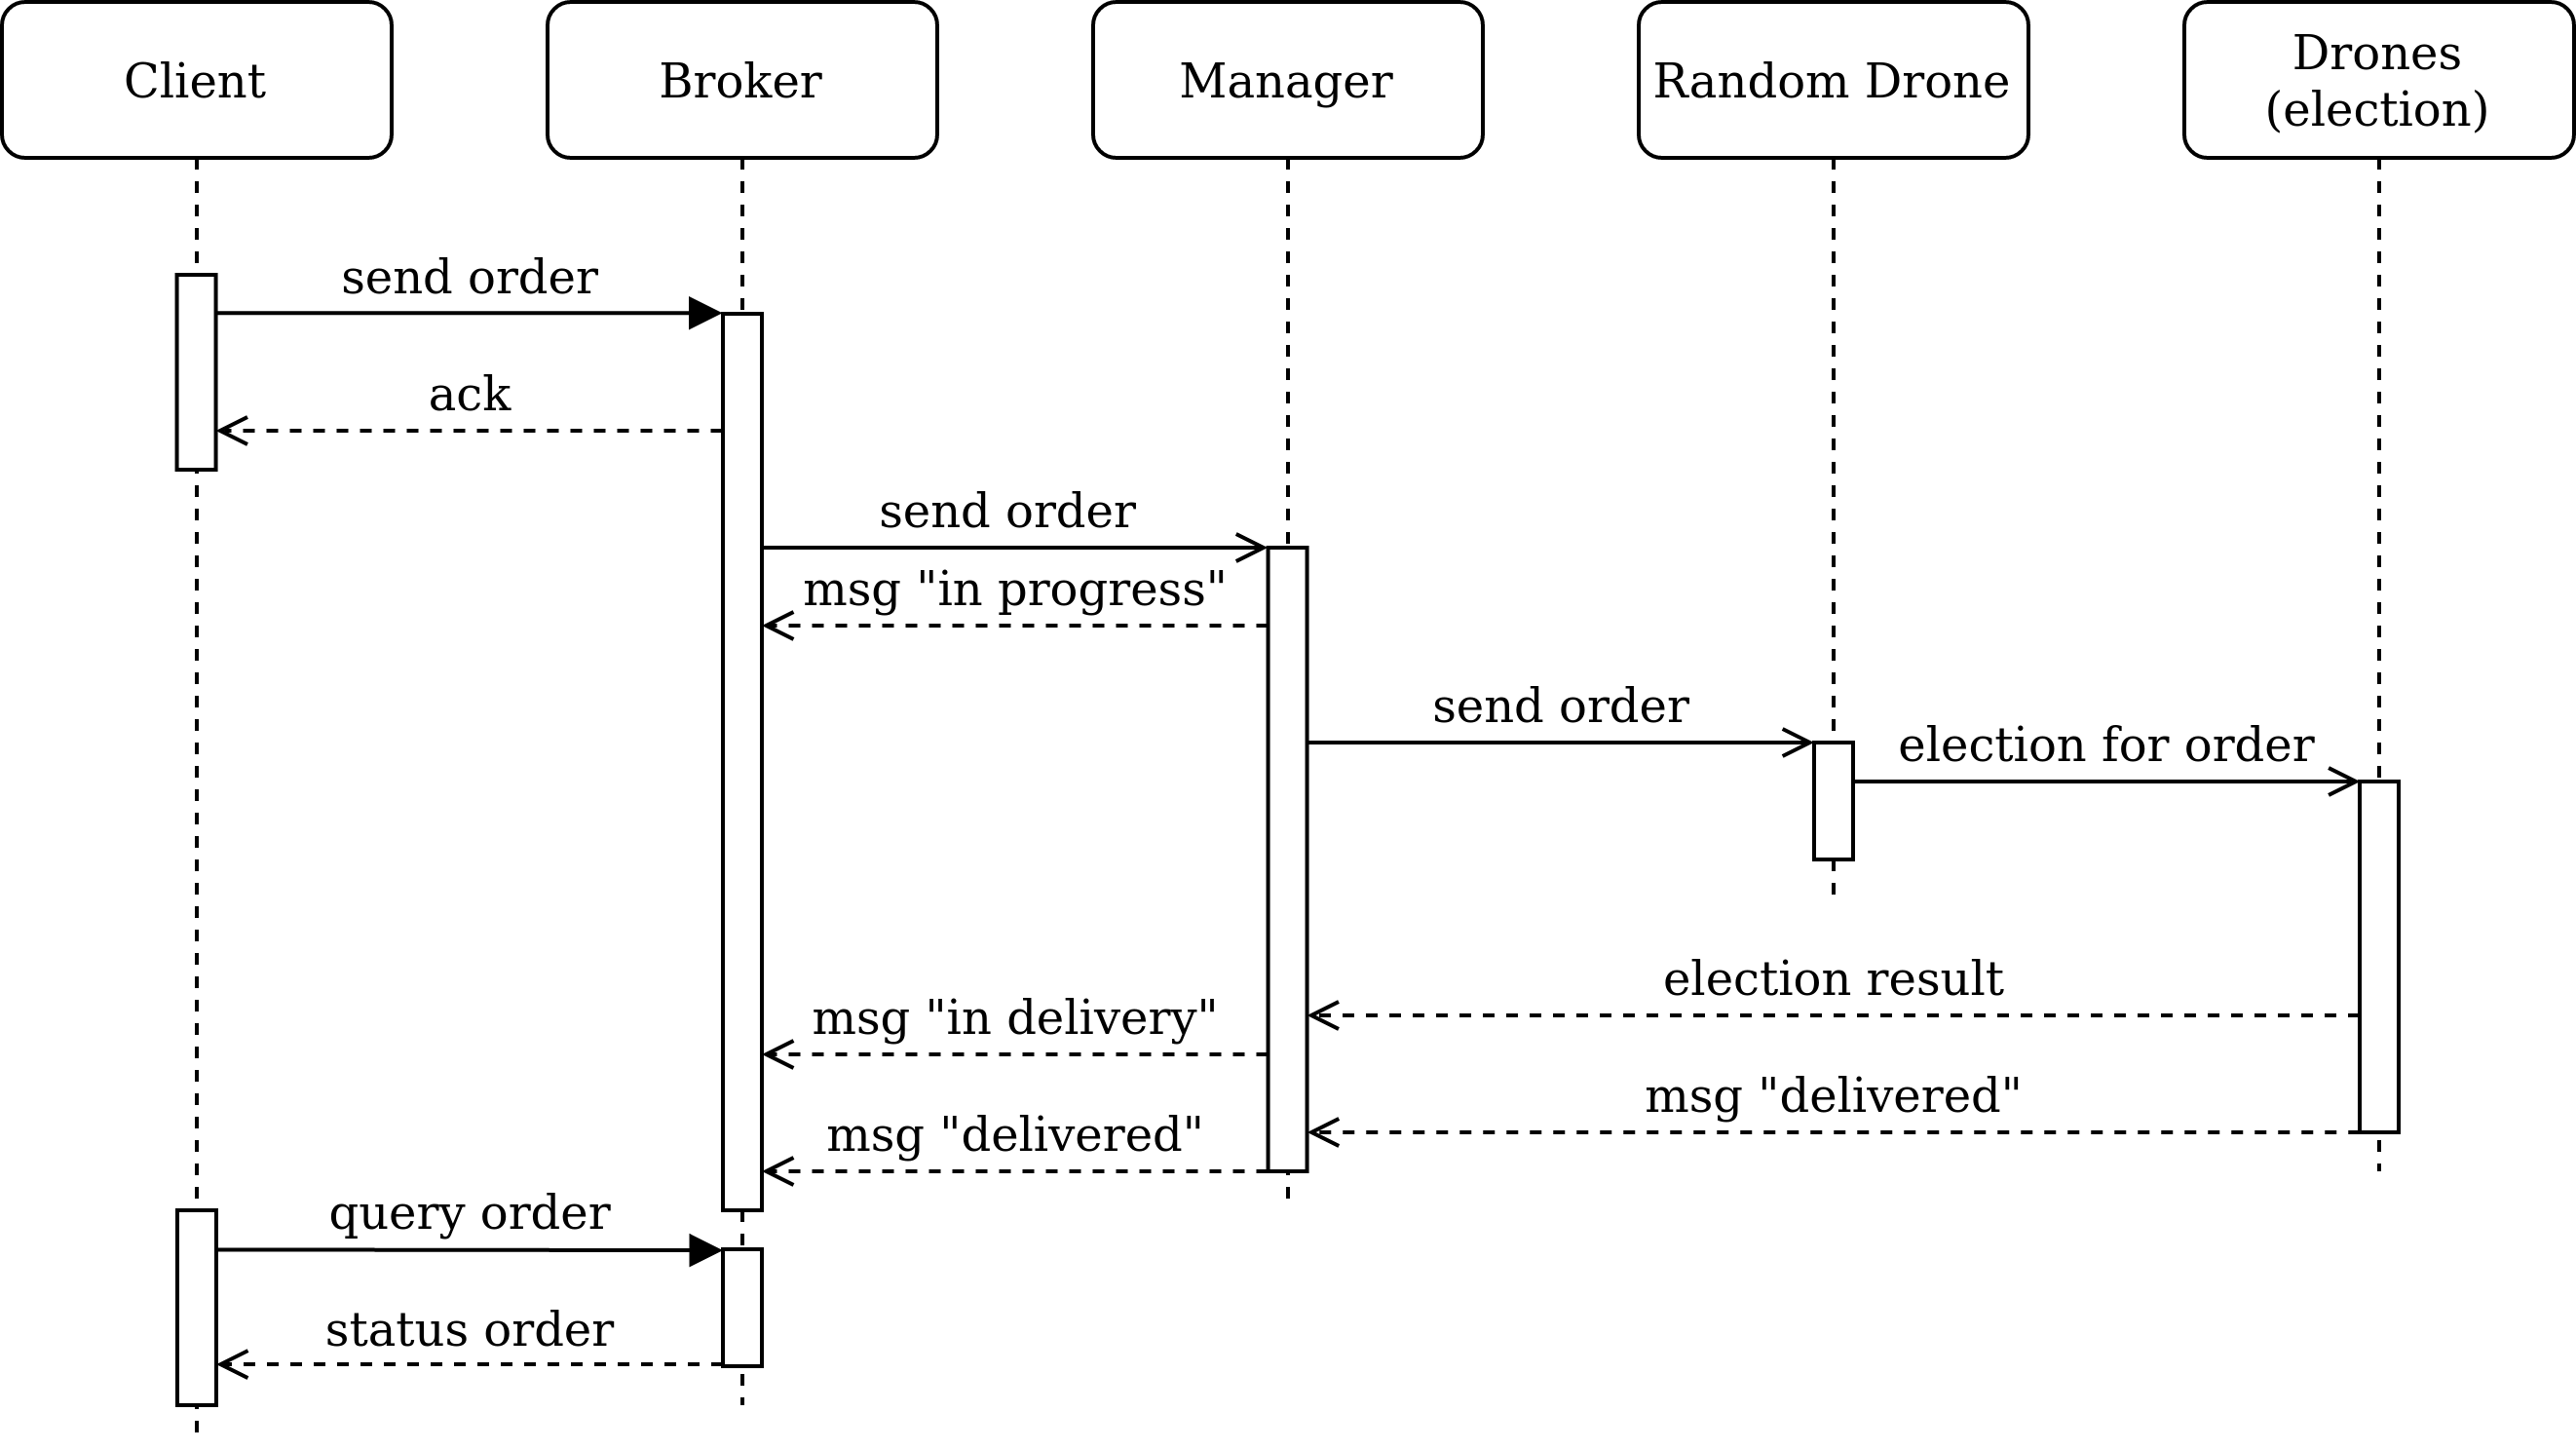
\includegraphics[width=\linewidth]{New-order}
	\caption{UML diagram for the execution of a delivery request}
\end{figure}

\subsection{Election behaviour}
In case of successful election the initiator will notify the elected drone, in the normal case the elected drone will notify the manager.
The elected drone could fail before receiving the message or silently discarding it because is already delivering a package. The manager will later inquire the situation.
\\\\
The election could fail due to multiple reasons:
\begin{enumerate}
	\item no drones available: conclude the election without notify the manager, the manager will later retry with a new election;
	\item no drones available with sufficient battery capacity: conclude the election, the manager will later retry with a new election, after 3 times a drone can't partecipate due to battery capacity, the drone will go to a recharging station;
	\item no drone available with sufficient weight capacity: conclude the election and notify the manager;
\end{enumerate}



Also, put here a detailed description of distributed algorithms used to solve specific problems of the project.

\section{Physical architecture and deployment}
%Which nodes and platforms involved, and where each component is deployed.
There are no specific requirements for the physical architecture, the drones can be deployed in any point of the map and the clients can request deliveries form and to any point in the map, the introduction of the broker and management servers for the network and order management enables the drones to be used only for the delivery of packages.


\section{Development plan}
The basic (tier 1) functionalities that the system must offer are:
\begin{itemize}
\item support for a dynamic number of clients and each one can make multiple delivery requests and query the broker for the status of the order;
\item broker and manager handle the orders and have a replica backup;
\item the fleet is made by a dynamic number of drones, they may fail; the drones carry the packages.
\end{itemize}

The extended (tier 2) functionalities are:
\begin{itemize}
\item support for failover and takeover of the servers;
\item instead of executing the various parts of the system on the same Erlang Machine, use containers to separate the various components of the system.
\item transportation of a broken drone to a repairing station;

\end{itemize}

%Since it is difficult to predict just how hard implementing a new system will be, you should formulate as a set of ``tiers,'' where the basic tier is something you’re sure you can complete, and the additional tiers add more features, at both the application and the system level.

\chapter{Implementation}

Details about the implementation: every choice about platforms, languages, software/hardware, middleware, which has not been decided in the requirements.


Important choices about implementation should be described here; e.g., peculiar data structures.

The storage of data relative to orders in the broker server and, drones and order in the manager server is done through the "Erlang Term Storage" (ETS) for the development mode with the purpose of preventing SSD consumption. In production the function calls should be substituted with the "Disk Erlang Term Storage" (DETS), an other option which require small changes is to use the Mnesia: the database included in Erlang, or some other database. In the development mode we choose the AVL tree as the data structure used by ETS over the hash table, without particular justification.

\chapter{Validation}
%Check if requirements from Chapter~\ref{ch:analysis} have been fulfilled.
%Quantitative tests (simulations) and screenshots of the interfaces are put here.

The system is according to the transparencies declared in the section \ref{System features}
\begin{itemize}
	\item \textbf{concurrency transparency}: the system must be able to handle multiple requests at the same time, this is done in such a way that every clients acts like if they were the only one making requests;
	\item \textbf{failure transparency}:the system manages faults of the drones and the servers in a transparent way: the broker and manager servers are synchronized with a backup server each that pings them and when the main server crashes the backup one will take its place, this way only a small part of the system will be disrupted, if a drone crashes another one will be selected to finish the delivery, it also removes the crashed drones from the drone table so they will not be candidates in other elections;
	\item \textbf{location transparency}: the client only needs to be able to connect with the broker server to request the delivery and to query the status of the request, it does not need to know which drones handle the request, their position or address or the physical position of the servers;
	\item \textbf{performance and scaling transparency}: the increase in the overall load on the network can be managed by increasing the number of drones in the network, the overhead of adding a new drone to the network is negligible. There is only one broker and one management server for the network and they can become bottlenecks, this could be solved by adding in the a proxy server that chooses the leader of the various broker servers;
	\item \textbf{reconfiguration transparency}: the structure of the network is not significantly impacted by the addition of a new drone, when a node crashes the network reconfigures itself in a transparent way for the client by removing the crashed drone from the drone table of the manager and the neighbour list of the other drones.
\end{itemize}


\chapter{Conclusions}

The possible extensions are:
\begin{itemize}
	\item realistic broker for large numbers of clients on multiple locations.
	\item Broker support for multiple manager servers for various fleets of drones.
	\item Support for warehouses, dynamic number of drones.
	\item Security concerns should be addressed, in all the parts of the system.
	\item The backup system could be improved with more servers, this can be achieved not by adding the backup server's addresses in the clients, but by a proxy server that choose the leader of the various broker servers. The broker servers can be configured with a master slave configuration or some more efficient solution like data partitioning. The proxy server can act as load balancer, accordingly to the configuration chosen.
\end{itemize}

Limit: scheduling performance.
\appendix

\chapter{Appendix}

In the Appendix you can put code snippets, snapshots, installation instructions, etc.


\chapter*{Evaluation}
Your system will be judged mainly on how it operates as a distributed system. The primary evaluation will be according to whether your system has the following attributes:
\begin{itemize}
\item  It should be an interesting distributed system, making use of some of the algorithms we have covered in class for distributed synchronization, replication, fault tolerance and recovery, security, etc.
\item The software should be well designed and well implemented, in terms of the overall architecture and the detailed realization.
\item You should devise and apply systematic testing procedures, at both the unit and systems levels.
\item The system should operate reliably and with good performance, even in the face of failures.
\end{itemize}
Important, but secondary considerations include:
\begin{itemize}
\item Time taken to do the project (the sooner the better, but do not miss details in order to end sooner)
\item  How nice is the application's appearance: does it have a nice interface or a compelling visual display?
\end{itemize}

\end{document}